Pour répondre au cahier des charges évoqué en introduction, nous avons choisi différents composants, voire plusieurs fois les mêmes. Nous allons expliciter nos choix dans la section ci-dessous :

\subsection{Raspberry Pi}
La Raspberry Pi a été cruciale dans notre projet en tant que cerveau central du robot. Elle a pris en charge la gestion des capteurs, la logique de contrôle, et les interactions avec les composants matériels. Grâce à sa connectivité GPIO, elle a permis une intégration facile avec les capteurs de suivi de ligne, les capteurs de distance, et d'autres périphériques. De plus, la possibilité de programmer en langage C a facilité le développement du logiciel embarqué car nous suivions en parallèle un cours sur ce même langage.

\begin{figure}[h]
    \centering
    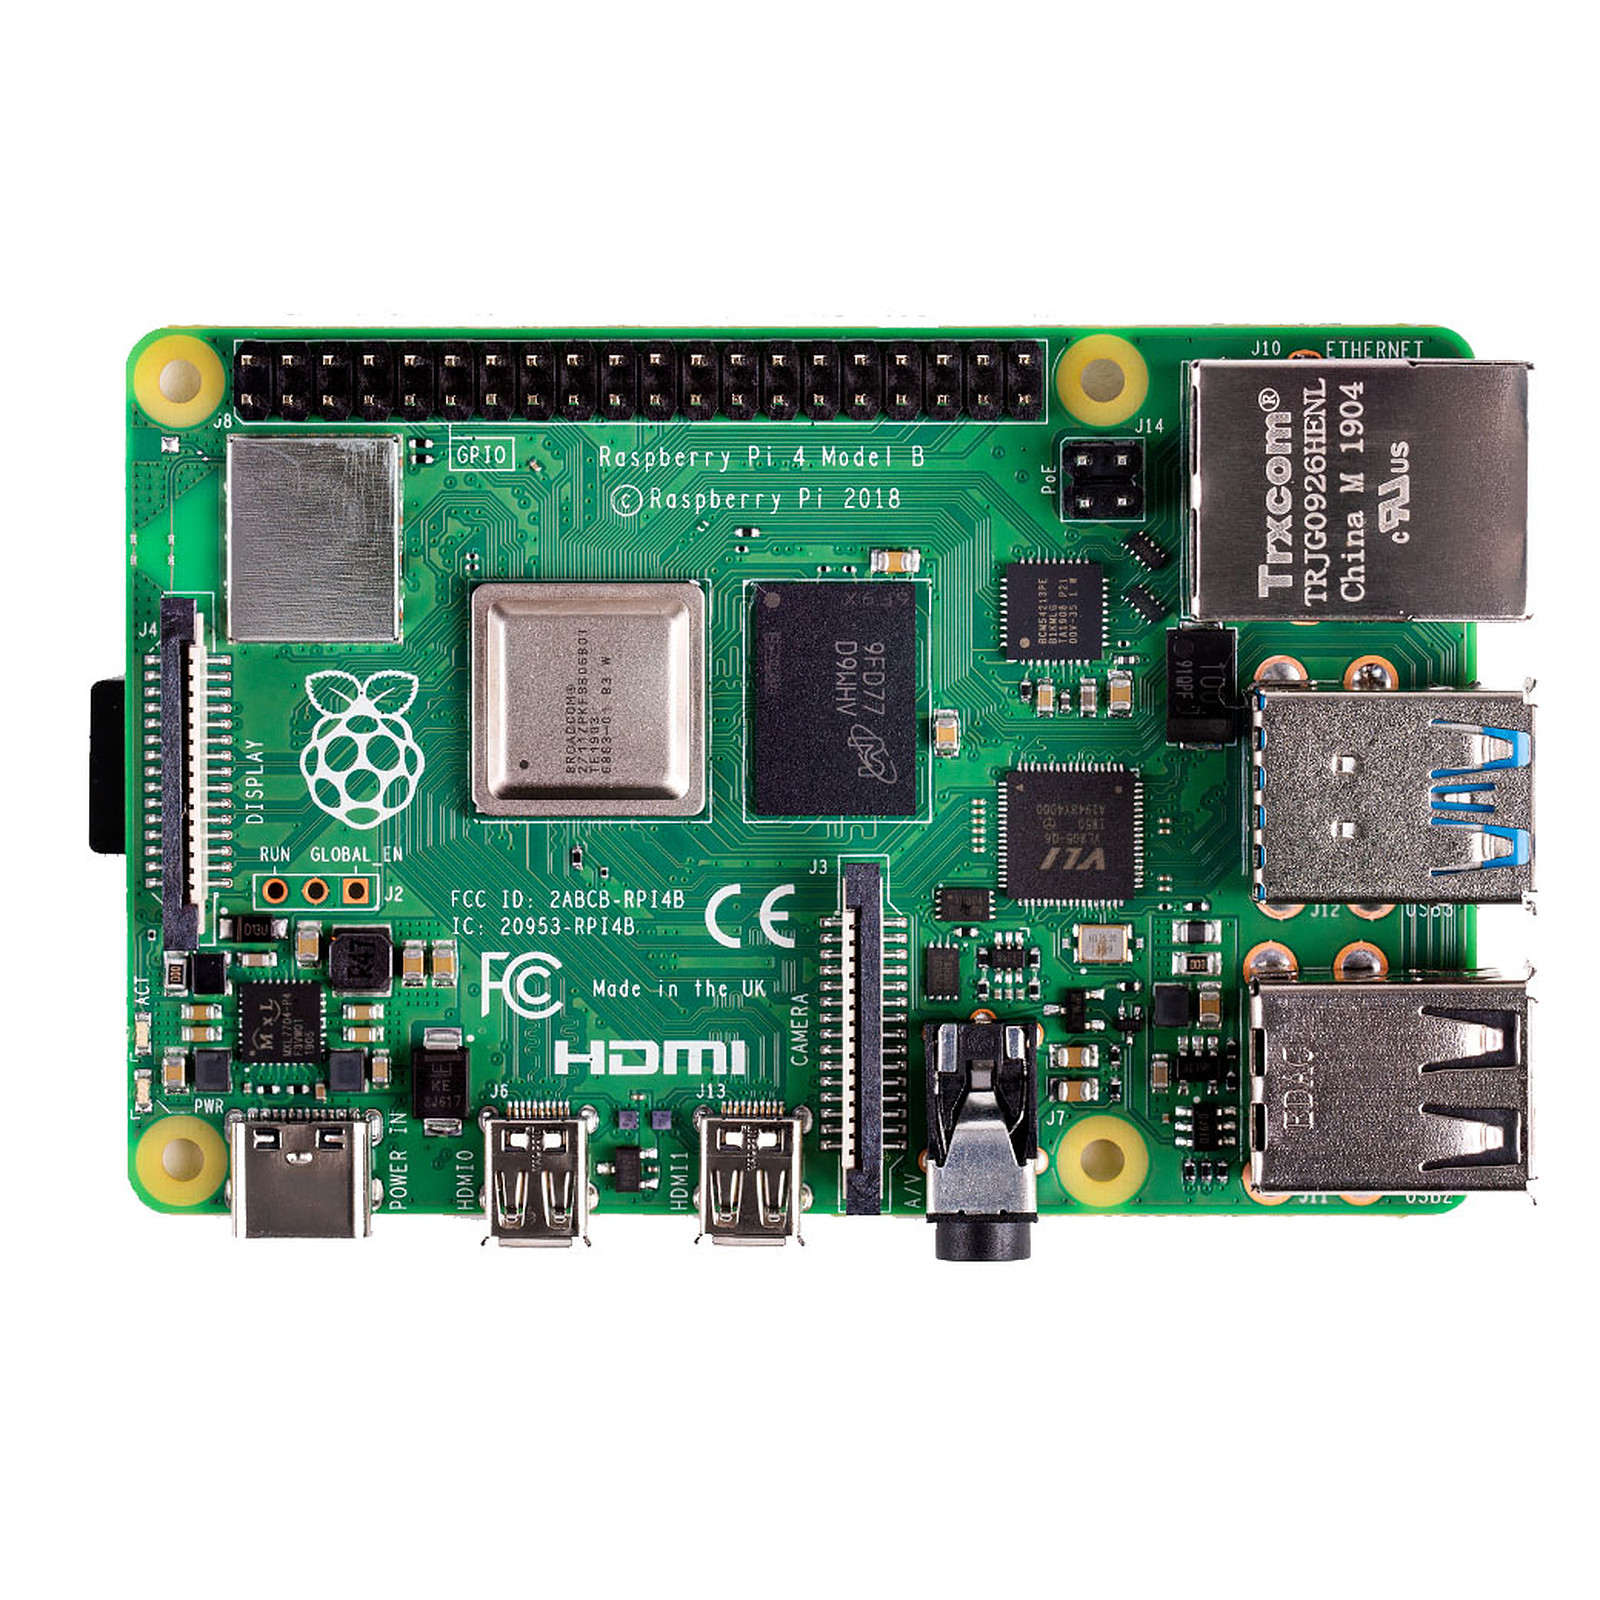
\includegraphics[width=0.3\textwidth]{components/RPi4.jpg}
    \caption{Raspberry Pi 4}
    \label{fig:Raspberry Pi 4}
\end{figure}

\subsection{Capteur infrarouge TCRT5000}
Les capteurs infrarouge, tels que le modèle TCRT5000 que nous avons choisi, jouent un rôle essentiel en tant que suiveurs de ligne dans notre robot. Leur principe de fonctionnement repose sur l'émission d'un faisceau infrarouge et la détection du signal réfléchi. Ce capteur est composé d'une LED infrarouge et d'un phototransistor, permettant de mesurer l'intensité du signal réfléchi. En suivant une ligne, le capteur détecte les variations d'intensité du signal infrarouge en fonction de la surface rencontrée, ce qui permet au robot de maintenir sa trajectoire ou non.

En effet, dans notre cas, nous avons utilisé trois suiveurs de ligne : un à gauche, un central et un à droite. Cela permet de couvrir toute la zone nécessaire pour suivre la ligne, détecter les intersections et tourner efficacement.

Dans un premier temps, il faut savoir que nous avons travaillé avec un autre type de capteur infrarouge suiveur de ligne plus compact mais moins performant. Cela n'a eu aucune conséquence sur la suite du projet car leur fonctionnement est quasiment similaires aux capteurs utilisés.

Le choix du capteur infrarouge s'aligne parfaitement avec les exigences du cahier des charges initial. Leur facilité d'intégration avec le Raspberry Pi, combinée à leur réactivité, offre une solution fiable pour le suivi de ligne, permettant au robot de naviguer de manière fluide tout en respectant les intersections définies dans le cahier des charges.

\begin{figure}[h]
    \centering
    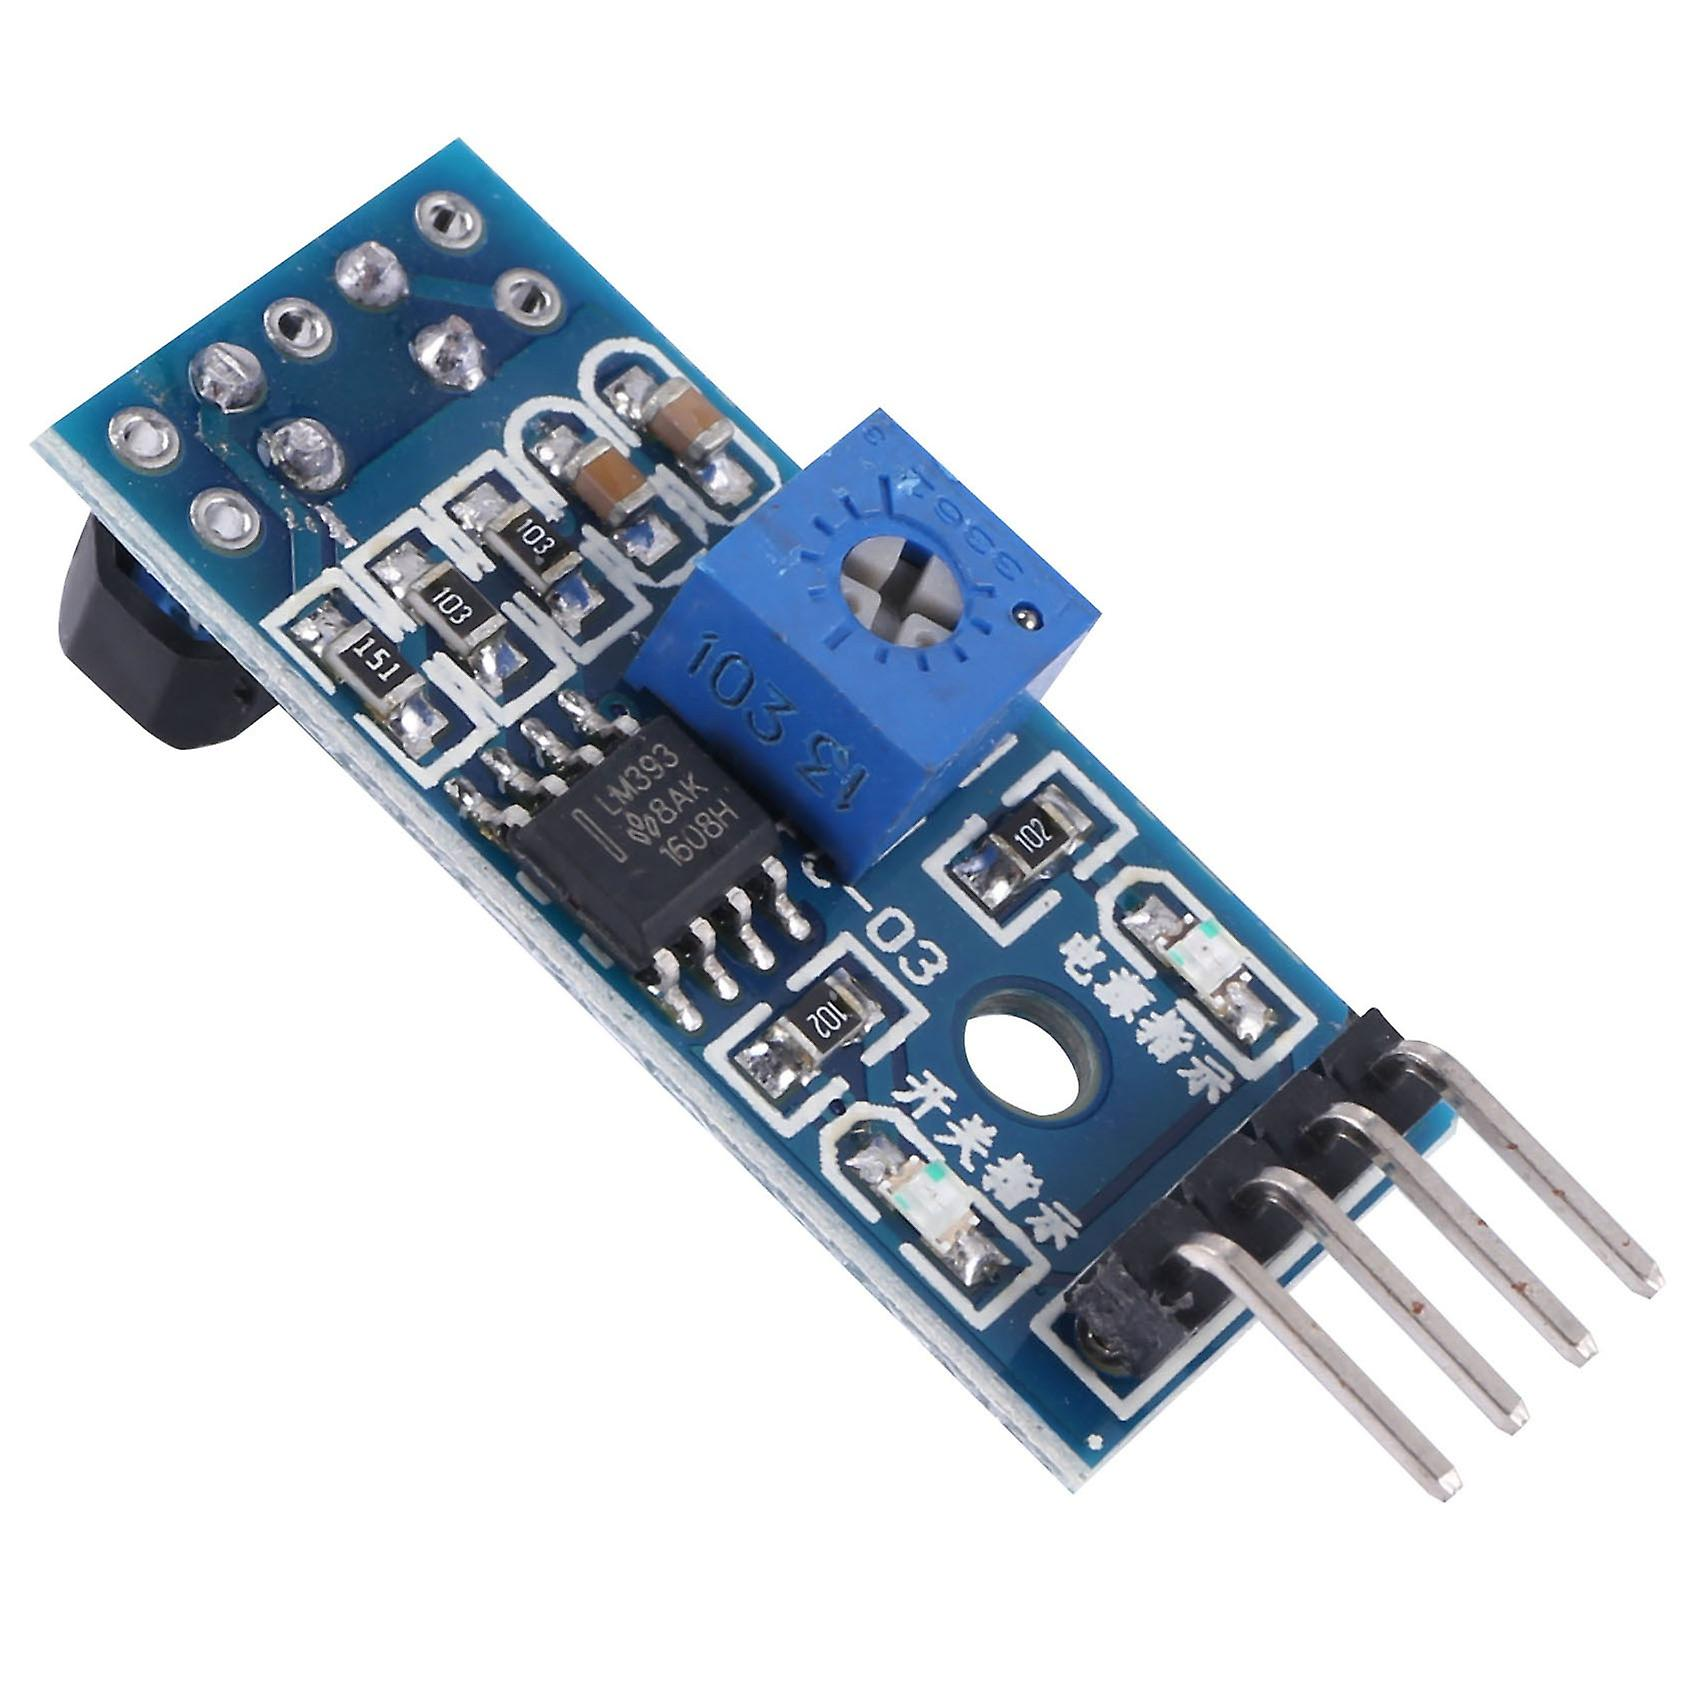
\includegraphics[width=0.3\textwidth]{components/line_finder.jpg}
    \caption{Capteur infrarouge de suivi de ligne TCRT5000}
    \label{fig:TCRT5000}
\end{figure}

\subsection{Moteurs et L293D}
Les moteurs directement reliés aux roues de notre robot constituent le cœur de sa mobilité.

Pour assurer un contrôle précis et bidirectionnel de ces moteurs, nous avons choisi d'utiliser la carte de commande de moteurs L293D. Cette carte offre une interface simple mais efficace entre le Raspberry Pi et les moteurs, permettant de réguler la vitesse et la direction de manière précise. Le L293D fonctionne en amplifiant les signaux de commande du Raspberry Pi pour fournir une alimentation adéquate aux moteurs, facilitant ainsi le contrôle des mouvements du robot.

La sélection du L293D s'inscrit parfaitement dans les exigences spécifiées dans notre cahier des charges initial. Sa capacité à gérer deux moteurs simultanément, à inverser la direction de rotation, et à ajuster la vitesse répond à notre besoin de contrôle moteur bidirectionnel pour le suivi de ligne et les manœuvres aux intersections.

À préciser qu'au début du projet, nous avons utilisé une carte MAKERDRIVE qui nous a posé beaucoup trop de problèmes à nous et à d'autres groupes ce qui a justifié notre changement vers la L293D. (Cela sera détaillé dans la partie 6. Difficultés rencontrées)

\begin{figure}[h]
    \centering
    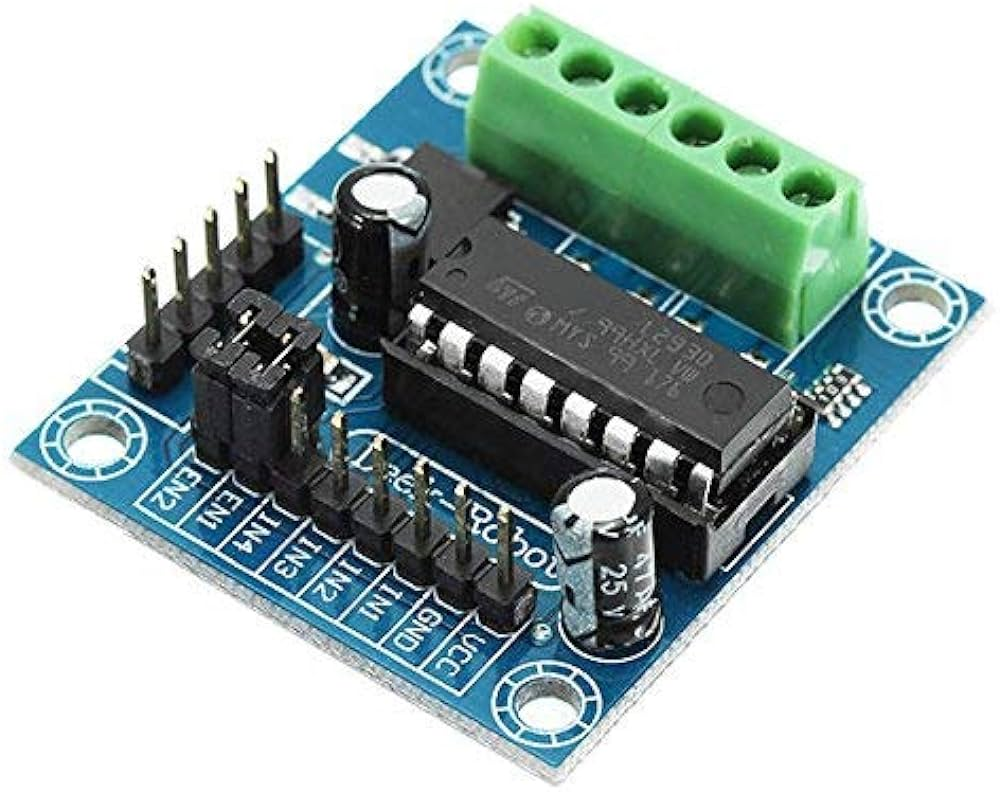
\includegraphics[width=0.3\textwidth]{components/L293D.jpg}
    \caption{Carte de contrôle des moteurs L293D}
    \label{fig:L293D}
\end{figure}

\subsection{Capteur ultrasons HS-SR04}
Les capteurs ultrasons, tels que le modèle HS-SR04 que nous avons intégré à notre robot, jouent un rôle crucial dans la détection des obstacles et la mesure de la distance frontale. Grâce à leur principe de fonctionnement, émettant des ondes sonores et mesurant le temps nécessaire à leur retour après réflexion sur un obstacle, ces capteurs fournissent une estimation précise de la distance entre le robot et tout objet présent sur sa trajectoire.

Le choix du capteur ultrasonique HS-SR04 découle directement des exigences spécifiées dans notre cahier des charges initial. Sa portée étendue et sa résolution précise permettent au robot de détecter les obstacles à des distances variées, contribuant ainsi à l'alerte précoce et à la prise de décision en temps réel. Cette fonctionnalité est essentielle pour respecter les critères du cahier des charges, notamment l'alerte en cas d'obstacle, l'arrêt d'urgence, et l'attente en présence d'obstacles.

\begin{figure}[h]
    \centering
    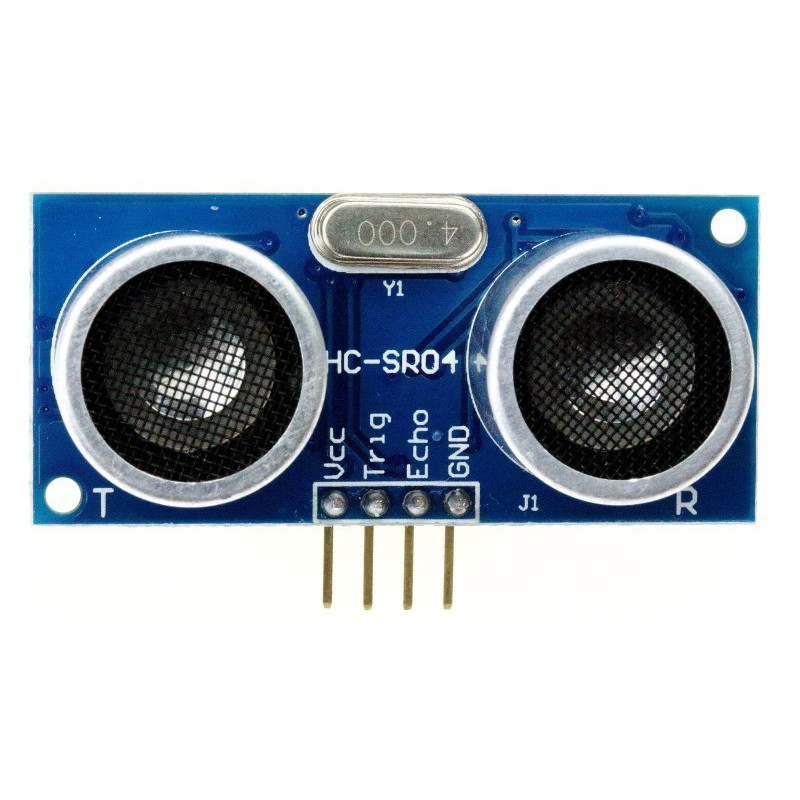
\includegraphics[width=0.3\textwidth]{components/capteur_ultrason.jpg}
    \caption{Capteur ultrasons HS-SR04}
    \label{fig:HS-SR04}
\end{figure}

\subsection{Active buzzer}
L'Active Buzzer, le composant d'alerte d'obstacle est essentiel pour notre robot suiveur de ligne. Conformément aux exigences énoncées dans notre cahier des charges initial, l'Active Buzzer est activé dès qu'un obstacle est détecté par les capteurs ultrasons. Cette alerte sonore, combinée à l'affichage sur l'écran LCD, permet d'assurer une notification immédiate de la proximité d'un objet.

\begin{figure}[h]
    \centering
    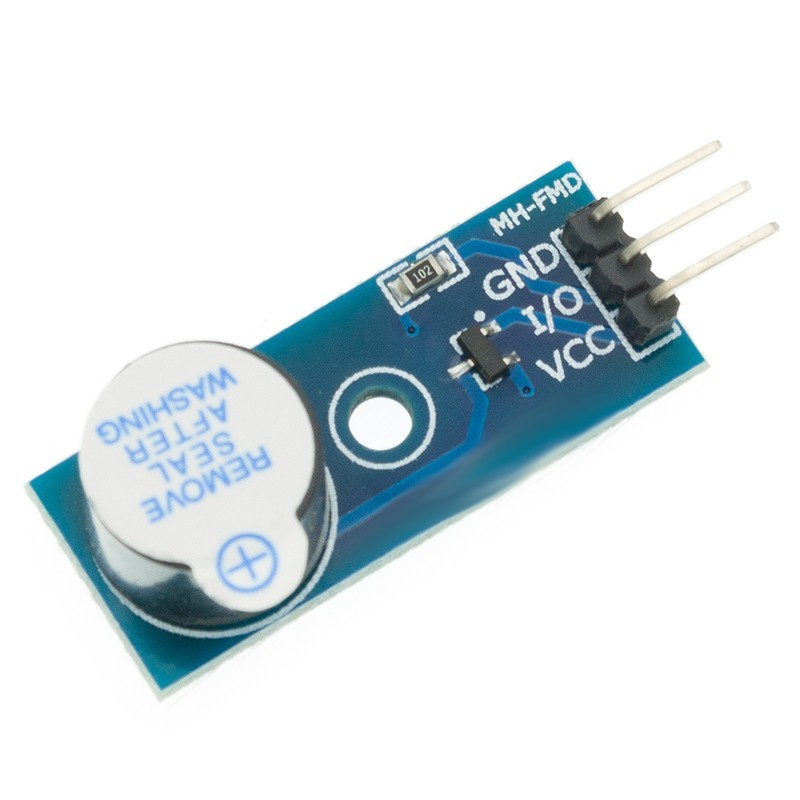
\includegraphics[width=0.3\textwidth]{components/active_buzzer.jpg}
    \caption{Active Buzzer}
    \label{fig:Active Buzzer}
\end{figure}

\subsection{LCD1602 et I2C Interface Module}
L'écran LCD1602, contrôlé via l'interface I2C, représente un élément central dans notre robot suiveur de ligne en fournissant une interface visuelle pour afficher des informations cruciales conformes aux spécifications du cahier des charges initial. Sa capacité à présenter en temps réel les mouvements programmés du robot, les distances mesurées par les capteurs, ainsi que l'état de connexion de la manette, offre une visibilité immédiate sur le statut opérationnel du robot. L'utilisation de l'I2C simplifie la connectivité entre l'écran LCD et le Raspberry Pi, permettant une intégration aisée dans notre système embarqué.

\begin{comment}
\begin{figure}[h]
    \centering
    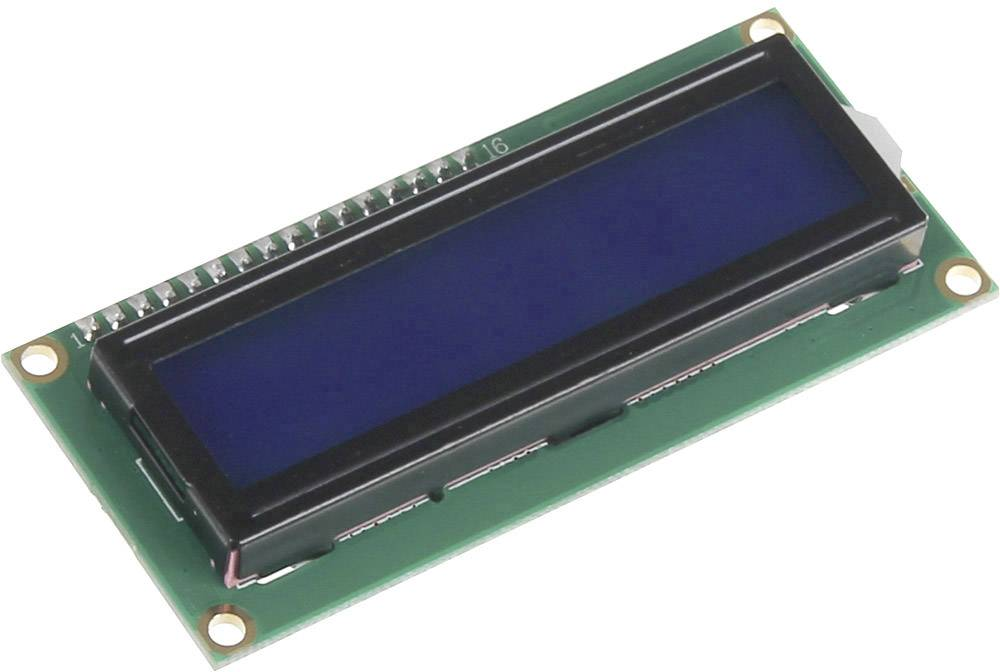
\includegraphics[width=0.4\textwidth]{components/LCD.jpg}
    \caption{Ecran LCD 1602}
    \label{fig:LCD1602}
\end{figure}
\end{comment}

\newpage

\subsection{Manette de PS5}
La manette de PS5 connectée en Bluetooth, avec sa configuration ergonomique et ses fonctionnalités avancées, offre une expérience de contrôle fluide et réactive. Les opérateurs peuvent ainsi ajuster la trajectoire du robot, effectuer des arrêts d'urgence, et contrôler manuellement les mouvements, répondant ainsi aux critères de contrôlabilité et d'interactivité définis dans le cahier des charges. En choisissant cette approche, notre robot suiveur de ligne intègre une solution de commande manuelle moderne et accessible, alignée sur les attentes spécifiées dès le début de notre projet. À noter que nous avons utilisé une manette de PS5 mais nous aurions pu utiliser quasiment n'importe quelle manette similaire. (Ceci a été détaillé plus haut dans la section 4.)

\begin{comment}
\begin{figure}[h]
    \centering
    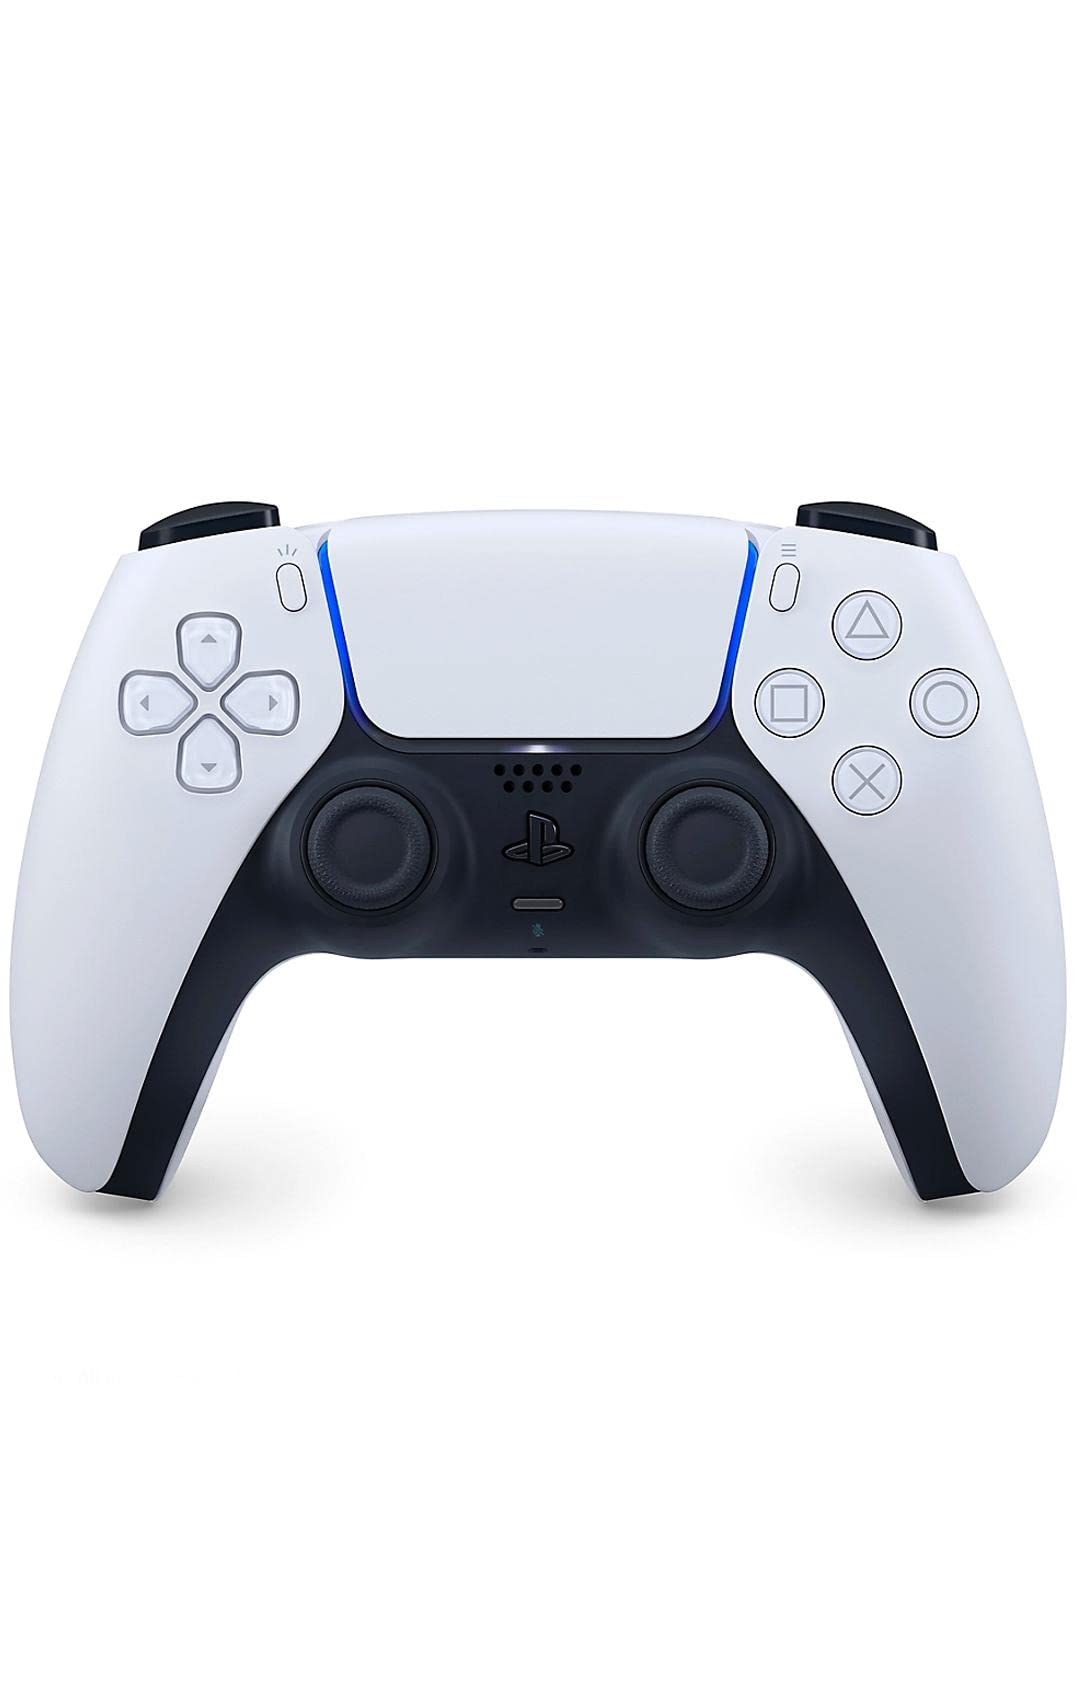
\includegraphics[width=0.2\textwidth]{components/manette_ps5.jpg}
    \caption{Manette de PS5}
    \label{fig:Manette de PS5}
\end{figure}
\end{comment}

\bigbreak
\begin{figure}[h]
    \begin{minipage}[c]{.46\linewidth}
        \centering
        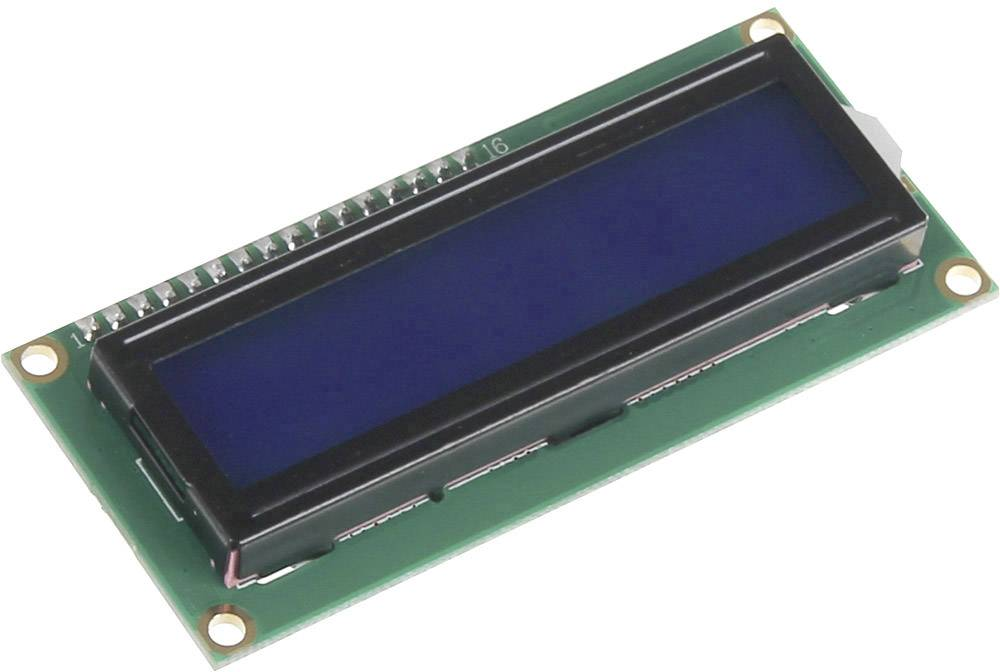
\includegraphics[width=0.5\textwidth]{components/LCD.jpg}
        \caption{Ecran LCD 1602}
        \label{fig:LCD1602}
    \end{minipage}
    \hfill%
    \begin{minipage}[c]{.46\linewidth}
        \centering
        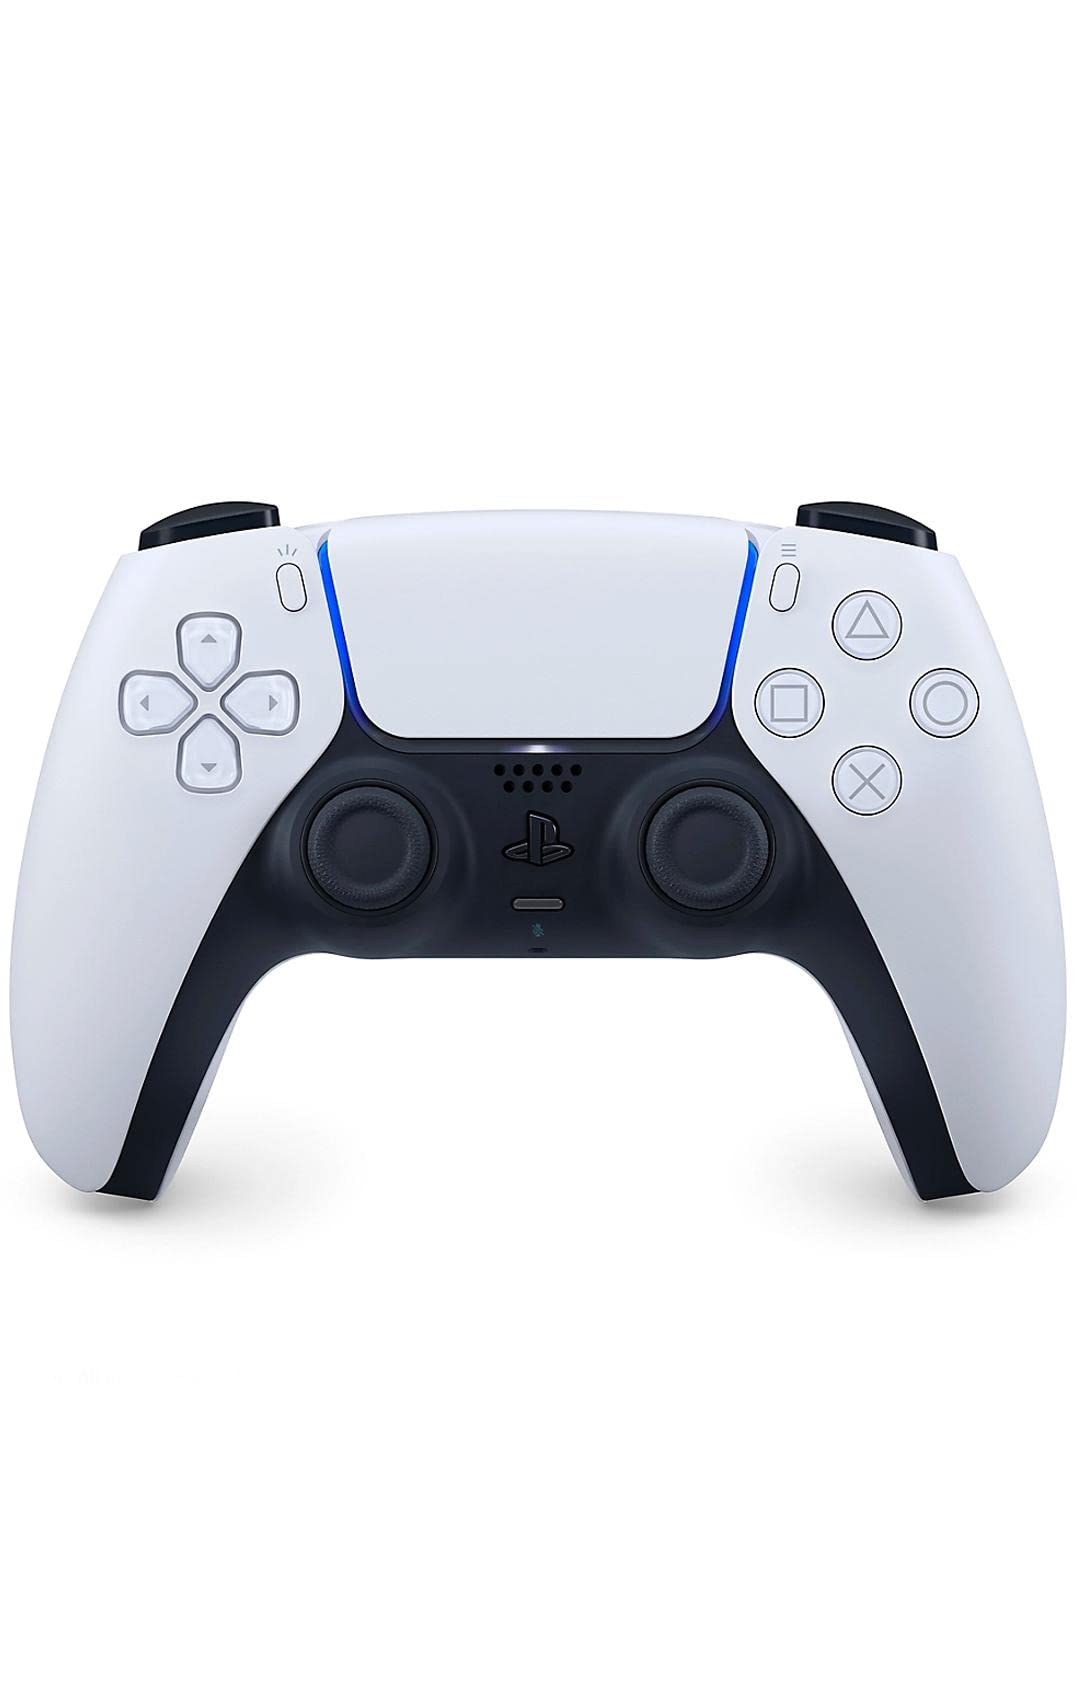
\includegraphics[width=0.5\textwidth]{components/manette_ps5.jpg}
        \caption{Manette de PS5}
        \label{fig:Manette de PS5}
    \end{minipage}
\end{figure}

\newpage